\documentclass[runningheads,orivec]{llncs}

\let\proof\relax %To avoid incompatibility between llncs and amsthm
\let\endproof\relax %To avoid incompatibility between llncs and amsthm
\let\proofname\relax %To avoid incompatibility between llncs and ntheorem


%\usepackage[hidelinks]{hyperref}
\usepackage{amsmath,amssymb,mathtools,stmaryrd}
\usepackage[amsthm,hyperref,thmmarks]{ntheorem}
\usepackage{marvosym}
\usepackage{nicefrac}

%\usepackage{fullpage}

\usepackage{xcolor}
\usepackage{tikz}
  \usetikzlibrary{arrows.meta}
  \usetikzlibrary{calc}
  \usetikzlibrary{matrix}
\usepackage{proof}

% Hyperlinks

\makeatletter
\RequirePackage[bookmarks,unicode,colorlinks=true]{hyperref}%
\def\@citecolor{blue}%
\def\@urlcolor{blue}%
\def\@linkcolor{blue}%
\def\UrlFont{\rmfamily}
\def\orcidID#1{\smash{\href{http://orcid.org/#1}{\protect\raisebox{-1.25pt}{\protect\includegraphics{orcid_color.eps}}}}}

%% theorem environments
\usepackage{cleveref}

\theoremstyle{definition}
\newtheorem{defn}{Definition}
\newtheorem{rmrk}[defn]{Remark}
%%
\theoremstyle{plain}
\newtheorem{conj} [defn]{Conjecture}
\newtheorem{cor}  [defn]{Corollary}
\newtheorem{lem}  [defn]{Lemma}
\newtheorem{prop} [defn]{Proposition}
\newtheorem{thm}  [defn]{Theorem}
\newtheorem{lemmaAppendix}{Lemma}
%%

%text
\newcommand{\eg}{\textit{e.g.}}
\newcommand{\ie}{\textit{i.e.}}
\newcommand{\ih}{\textit{i.h.}}

% coloneqq
\newcommand*\coloneq{
 \mathrel{%
  \rlap{\raisebox{0.3ex}{$\m@th\cdot$}}%
        \raisebox{-0.3ex}{$\m@th\cdot$}%
 {=}}}
\newcommand*\coloneqq{
 \mathrel{%
  \rlap{\raisebox{0.3ex}{$\m@th\cdot$}}%
        \raisebox{-0.3ex}{$\m@th\cdot$}%
  \rlap{\raisebox{0.3ex}{$\m@th\cdot$}}%
        \raisebox{-0.3ex}{$\m@th\cdot$}%
 {=}}}

% vcenter
\newcommand\vc[1]{\vcenter{\hbox{$#1$}}}

% Small operators:

\newcommand\smallbin[1]{\mathchoice
      {\mathbin{\raise.2ex \hbox{$\scriptstyle      #1$}}}%
      {\mathbin{\raise.2ex \hbox{$\scriptstyle      #1$}}}%
      {\mathbin{\raise.12ex\hbox{$\scriptscriptstyle#1$}}}%
      {\mathbin{           \hbox{$\scriptscriptstyle#1$}}}}%

\newcommand\smallsquare{\mathchoice{{\scriptstyle\square}}{{\scriptstyle\square}}{{\scriptscriptstyle\square}}{{\scriptscriptstyle\square}}}

\newcommand\Con{\wedge}
\newcommand\Imp{\rightarrow}

\newcommand\con{\kern1pt{\smallbin\Con}\kern1pt}
\newcommand\imp{\kern1pt{\smallbin\Imp}}


% ===== TERMS AND TYPES

% Probabilistic lambda-calculus
\newcommand\PEL{\Lambda_{\textsf{PE}}}

% Free variables
\newcommand\fv[1]{\mathsf{fv}(\trm{#1})}
\newcommand\fl[1]{\mathsf{fl}(\trm{#1})}

% colours
\colorlet{mgray}{black!40}
\colorlet{lgray}{black!25}
\colorlet{llgray}{black!15}

\colorlet{dblue}{blue!80!black}
\colorlet{dred}{red!80!black}

\colorlet{typecolor}{dblue}
\colorlet{termcolor}{dred}

\newcommand\typecolor{\color{typecolor}}
\newcommand\termcolor{\color{termcolor}}

\newcommand\black{\color{black}}
\newcommand\dblue{\color{dblue}}
\newcommand\dred{\color{dred}}


% types
\newcommand\type[1]{{\let\type@sup@color\termcolor\typecolor\typ{#1}}}
\newcommand\typ[1]{%
  %\vphantom J%
  \let\type@loop=\type@next%
  \type@loop#1,%
}
\newcommand\type@next[1]{%
  \ifx#1,\let\type@loop\type@end\else%
  \ifx#1_\let\type@loop\type@sub\else%
  \ifx#1^\let\type@loop\type@sup\else%
  \ifx#1*\con\else%
  \ifx#1-\kern1pt{\imp}\else%
  #1%
  \fi\fi\fi\fi\fi%
  \type@loop%
}
\newcommand\type@sup@color{}
\newcommand\type@sub[1]{_{#1}\let\type@loop\type@next\type@loop}
\newcommand\type@sup[1]{^{{\type@sup@color #1}}\let\type@loop\type@next\type@loop}
\newcommand\type@vec[1]{\vec{\kern.5pt#1\kern.5pt}\let\type@loop\type@next\type@loop}
\newcommand\type@end{\let\type@sup@color\relax}

% terms
\newcommand\x{\lambda x}
\newcommand\y{\lambda y}
\newcommand\z{\lambda z}

\newcommand\+[1][{}]{\kern1pt{\smallbin\oplus}_{#1}\kern1pt}

\newcommand\1{\bullet}
\newcommand\0{\circ}

\newcommand{\full}{\bullet}

\newcommand\ttrm[1]{\smash{\trm{#1}}}

\newcommand\term[1]{{\let\term@typecolor\typecolor\termcolor\trm{#1}}}
\newcommand\trm[1]{%
  \vphantom(%
  \let\term@loop=\term@next%
  \term@loop#1,%
}
\newcommand\term@next[1]{%
  \ifx#1,\let\term@loop\term@end\else%
  \ifx#1:\black\colon\term@typecolor\let\term@loop\term@type\else%
  \ifx#1_\let\term@loop\term@sub\else%
  \ifx#1^\let\term@loop\term@sup\else%
  \ifx#1!\let\term@loop\term@box\else%
  \ifx#1+\let\term@loop\term@prob\else%
  \ifx#1*^\1\else%
  \ifx#1o_\1\else%
  \ifx#1p_\perm\else%
  \ifx#1q_{\1\perm}\else%
  \ifx#1i{\kern1pt}^i\else
  \ifx#1v\plusval\else%
  \ifx#1<\lfloor\else%
  \ifx#1>\rfloor\else%
  \ifx#1..\,\else%
  \ifx#1=\kern1pt{\smallbin=}\kern1pt\else
  #1%
  \fi\fi\fi\fi\fi\fi\fi\fi\fi\fi\fi\fi\fi\fi\fi\fi%\fi\fi\fi%
  \term@loop%
}
\newcommand\term@typecolor{}
\newcommand\term@end{\let\term@typecolor\relax}
\newcommand\term@sub[1]{_{#1}\let\term@loop\term@next\term@loop}
\newcommand\term@sup[1]{^{#1}\let\term@loop\term@next\term@loop}
\newcommand\term@vec[1]{\vec{\kern.5pt#1\kern.5pt}\let\term@loop\term@next\term@loop}
\newcommand\term@val[1]{\kern1pt\raisebox{-.5pt}{$\overset{\raisebox{-1pt}{$\scriptstyle#1$}}{{\smallbin\oplus_{\makebox[0pt][l]{$\scriptstyle\val$}}}}$}\kern5pt\let\term@loop\term@next\term@loop}
\newcommand\term@prob[1]{\kern1pt\raisebox{-.5pt}{$\overset{\raisebox{-1pt}{$\scriptstyle#1$}}{{\smallbin\oplus}}$}\kern1pt\let\term@loop\term@next\term@loop}
\newcommand\term@type{\let\type@loop=\type@next\type@loop}
\newcommand\term@box[1]{\probox{#1}\let\term@loop\term@next\term@loop}

\newcommand\probox[1]{\begin{tikzpicture}[baseline=0]\node[anchor=base](a){$\scriptstyle #1\vphantom)$};\draw[line width=.6pt] (-5pt,-2.5pt) rectangle (5pt,7.5pt);\end{tikzpicture}}

% judgments
\newcommand{\labjudg}[2]{#1\vdash_{L} #2}

\newcommand{\arrow}{\Rightarrow}
\newcommand{\judg}[3]{#1\vdash #2:#3}

% rewriting
\newcommand\rw[1][{}]{\stackrel{#1}\rightsquigarrow}
\newcommand\dw{\rotatebox[origin=c]{270}{$\rw$}}
\newcommand\lw{\rotatebox[origin=c]{180}{$\rw$}}
\newcommand\lrw{\rotatebox[origin=c]{180}{$\lw\!\rw$}}
\newcommand\perm{\mathsf p}
\newcommand\ph{{\pi{\mathsf h}}}

\newcommand\confluence[4]{\begin{array}{ccc} \trm{#1} & \rw & \trm{#2} \\ \dw && \dw \\ \trm{#3} & \rw & \trm{#4} \end{array}}

\newcommand\rstrut{\rule{0pt}{13pt}}

\newcommand\SN{\textsf{SN}}

\newcommand\proj[3]{\pi^{#1}_{#2}(\trm{#3})}

% strategies
\newcommand\cbn{\mathsf{cbn}}
\newcommand\cbv{\mathsf{cbv}}

\newcommand\val{\mathsf{v}}
\newcommand\plusval{\mathbin{\smallbin\oplus_\val}}

% translations
\newcommand\uncbv[1]{\llbracket#1\rrbracket_\val}
\newcommand\unopen[1]{\llbracket#1\rrbracket_{\mathsf{open}}}
\newcommand\labclose[2]{\lfloor\labjudg{#1}{#2}\rfloor}

% new rewriting

\tikzstyle{implied}=[dashed]
\tikzstyle{rwhead}=[>/.tip={Triangle[open,length=2.5pt,width=4.5pt]},|/.tip={Rectangle[length=.5pt,width=4.5pt]}]
\tikzstyle{rwblack}=[>/.tip={Triangle[length=2.5pt,width=4.5pt]},|/.tip={Rectangle[length=.5pt,width=4.5pt]}]
\tikzstyle{rw} =[line width=.5pt,rwhead,->]
\tikzstyle{rwb}=[line width=.5pt,rwblack,->]
\tikzstyle{rwbs}=[line width=.5pt,rwblack,->.>]
\tikzstyle{rws}=[line width=.5pt,rwhead,->.>]
\tikzstyle{rwn}=[line width=.5pt,rwhead,->.>|]
\tikzstyle{rwbn}=[line width=.5pt,rwblack,->.>|]
\tikzstyle{rwp}=[line width=.5pt,rwhead,->,double]
\tikzstyle{rwx}=[line width=.5pt,rwhead,->.>,double]

\renewcommand\rw{\mathrel{\tikz\draw[rw](0,0)--(10pt,0pt);}}
\newcommand\rwb{\mathrel{\tikz\draw[rwb](0,0)--(10pt,0pt);}}
\newcommand\rwbs{\mathrel{\tikz\draw[rwbs](0,0)--(10pt,0pt);}}
\newcommand\rws{\mathrel{\tikz\draw[rws](0,0)--(10pt,0pt);}}
\newcommand\rwn{\mathrel{\tikz\draw[rwn](0,0)--(10pt,0pt);}}
\newcommand\rwbn{\mathrel{\tikz\draw[rwbn](0,0)--(10pt,0pt);}}
\newcommand\rwp{\mathrel{\tikz\draw[rwp](0,0)--(10pt,0pt);}}
\newcommand\rwx{\mathrel{\tikz\draw[rwx](0,0)--(10pt,0pt);}}
\newcommand\rwps{\mathrel{\tikz\draw[rwx](0,0)--(10pt,0pt);}}

\newcommand\rwpleft{\mathrel{\tikz\draw[rwp](10pt,0pt)--(0,0);}}
\newcommand\rwxleft{\mathrel{\tikz\draw[rwx](10pt,0pt)--(0,0);}}
\newcommand\rwsleft{\mathrel{\tikz\draw[rws](10pt,0pt)--(0,0);}}

% rule names

\newcommand\idem{\ensuremath{\mathsf i}}
\newcommand\cancelL{\ensuremath{\mathsf c_1}}
\newcommand\cancelR{\ensuremath{\mathsf c_2}}
\newcommand\plusAbs{\ensuremath{{\smallbin\oplus}\lambda}}
\newcommand\plusArg{\ensuremath{{\smallbin\oplus}\mathsf a}}
\newcommand\plusFun{\ensuremath{{\smallbin\oplus}\mathsf f}}
\newcommand\plusBox{\ensuremath{{\smallbin{\oplus}\smallsquare}}}
\newcommand\plusL{\ensuremath{{\smallbin\oplus}{\smallbin\oplus}_1}}
\newcommand\plusR{\ensuremath{{\smallbin\oplus}{\smallbin\oplus}_2}}
\newcommand\plusX{\ensuremath{{\smallbin\oplus}{\star}}}
\newcommand\boxVoid{\ensuremath{\not{\kern-2pt\smallsquare}}}
\newcommand\boxAbs{\ensuremath{\smallsquare\lambda}}
\newcommand\boxFun{\ensuremath{\smallsquare\mathsf f}}


\makeatother

% reducibility

\newcommand{\RedSet}[1]{\mathit{Red}_{#1}}

% streams

\newcommand\Streams{\mathbb S}

% environments

\newenvironment{varitemize}
{
\begin{list}{\labelitemii}
{\setlength{\itemsep}{0pt}
 \setlength{\topsep}{0pt}
 \setlength{\parsep}{0pt}
 \setlength{\partopsep}{0pt}
 \setlength{\leftmargin}{15pt}
 \setlength{\rightmargin}{0pt}
 \setlength{\itemindent}{0pt}
 \setlength{\labelsep}{5pt}
 \setlength{\labelwidth}{10pt}
}}
{
 \end{list}
}

%============================================================ FRONTMATTER

\title{Decomposing Probabilistic Lambda-Calculi}


\author{
	 Ugo Dal Lago\inst{1}\orcidID{0000-0001-9200-070X}
\and Giulio Guerrieri\inst{2}\textsuperscript{(\Letter)}\orcidID{0000-0002-0469-4279}
\and Willem Heijltjes\inst{2}
}

\authorrunning{U.\ Dal Lago, G.\ Guerrieri, and W.\ Heijltjes}

\institute{%
	Dipartimento di Informatica - Scienza e Ingegneria
\\	Universit\`a di Bologna, Bologna, Italy
\\	\email{ugo.dallago@unibo.it}
\\[10pt]\and%
	Department of Computer Science
\\	University of Bath, Bath, UK
\\	\email{\{w.b.heijltjes,g.guerrieri\}@bath.ac.uk}
}



%============================================================ DOCUMENT

\begin{document}

\maketitle

\begin{abstract}
A notion of probabilistic lambda-calculus usually comes with a prescribed reduction strategy, typically call-by-name or call-by-value, as the calculus is non-confluent and these strategies yield different results. This is a break with one of the main advantages of lambda-calculus: confluence, which means results that are independent from the choice of strategy.
We present a probabilistic lambda-calculus where the probabilistic operator is decomposed into two syntactic constructs: a generator, which represents a probabilistic event; and a consumer, which acts on the term depending on a given event. The resulting calculus, the Probabilistic Event Lambda-Calculus, is confluent, and interprets the call-by-name and call-by-value strategies through different interpretations of the probabilistic operator into our generator and consumer constructs.
We present two notions of reduction, one via fine-grained local rewrite steps, and one by generation and consumption of probabilistic events. Simple types for the calculus are essentially standard, and they convey strong normalization. We demonstrate how we can encode call-by-name and call-by-value probabilistic evaluation.
\end{abstract}

\section{Introduction}

Probabilistic lambda-calculi \cite{SahebDjahromi78,Manber-Tompa-1982,JonesPlotkin89,deLiguoroPiperno95,JungTix98,DalLagoZorzi12,FaggianRonchi19} extend the standard lambda-calculus with a probabilistic choice operator $N\+[p]M$, which chooses $N$ with probability $p$ and $M$ with probability $1-p$ (throughout this paper, we let $p$ be $\nicefrac12$ and will omit it). Duplication of $N\+M$, as is wont to happen in lambda-calculus, raises a fundamental question about its semantics: do the duplicate occurrences represent \emph{the same} probabilistic event, or \emph{different} ones with the same probability? For example, take the term $\top\+\bot$ that represents a coin flip between boolean values \emph{true} $\top$ and \emph{false} $\bot$. If we duplicate this term, do the copies represent two distinct coin flips with possibly distinct outcomes, or do these represent a single coin flip that determines the outcome for both copies? Put differently again, when we duplicate $\top\+\bot$, do we duplicate the \emph{event}, or only its \emph{outcome}?

In probabilistic lambda-calculus, these two interpretations are captured by the evaluation strategies of call-by-name ($\rw_\cbn$), which duplicates events, and call-by-value ($\rw_\cbv$), which evaluates any probabilistic choice before it is duplicated, and thus only duplicates outcomes. Consider the following example, where $=$ tests equality of boolean values.
\[
	\top \quad {}_\cbv\!\rwsleft \quad (\x.\,x = x)(\top\+\bot) \quad \rws_\cbn \quad \trm{\top\+\bot}
\]
This situation is not ideal, for several, related reasons. Firstly, it demonstrates how probabilistic lambda-calculus is non-confluent, negating one of the central properties of the lambda-calculus, and one of the main reasons why it is the prominent model of computation that it is. Secondly, it means that a probabilistic lambda-calculus must derive its semantics from a prescribed reduction strategy, and its terms only have meaning in the context of that strategy. Thirdly, combining different kinds of probabilities becomes highly involved~\cite{FaggianRonchi19}, as it would require specialized reduction strategies. These issues present themselves even in a more general setting, namely that of commutative (algebraic) effects, which in general do not commute with copying.

We address these issues by a decomposition of the probabilistic operator into a \emph{generator} $\ttrm{!a}$ and a \emph{choice} $\ttrm{+a}$, as follows.
\[
	\trm{N \+ M} \quad\stackrel\Delta=\quad \trm{!a. N +a M}
\]
Semantically, $\ttrm{!a}$ represents a probabilistic event, that generates a boolean value recorded as $a$. The choice $\ttrm{N+aM}$ is simply a conditional on $a$, choosing $N$ if $a$ is false and $M$ if $a$ is true. Syntactically, $a$ is a boolean variable with an occurrence in $\ttrm{+a}$, and $\ttrm{!a}$ acts as a probabilistic quantifier, binding all occurrences in its scope. (To capture a non-equal chance, one would attach a probability $p$ to a generator, as $\ttrm{!a}{\kern1pt}_p$, though we will not do so in this paper.)

The resulting \emph{probabilistic event lambda-calculus} $\PEL$, which we present in this paper, is confluent. Our decomposition allows us to separate duplicating an \emph{event}, represented by the generator $\ttrm{!a}$, from duplicating only its \emph{outcome} $a$, through having multiple choice operators $\trm{+a}$. In this way our calculus may interpret both original strategies, call-by-name and call-by-value, by different translations of standard probabilistic terms into $\PEL$: call-by-name by the above decomposition (see also Section~\ref{sec:PEL}), and call-by-value by a different one (see Section~\ref{sec:cbv}). For our initial example, we get the following translations and reductions.
%
\begin{alignat}{3}
\cbn: \quad & \trm{(\x.x = x)(!a.\top+a\bot)} & \quad \rw_\beta \quad & \trm{(!a.\top+a\bot)=(!b.\top+b\bot)} & \quad \rws \quad & \top\+\bot \label{eq:cbn}
\\
\cbv: \quad & \trm{!a.(\x.x = x)(\top+a\bot)} & \quad \rw_\beta \quad & \trm{!a.(\top+a\bot)=(\top+a\bot)}    & \quad \rws \quad & \top \label{eq:cbv}
\end{alignat}

We present two reduction relations for our probabilistic constructs, both independent of beta-reduction. Our main focus will be on \emph{permutative} reduction (Sections~\ref{sec:PEL},~\ref{sec:p-reduction}), a small-step local rewrite relation which is computationally inefficient but gives a natural and very fine-grained operational semantics. \emph{Projective} reduction (Section~\ref{sec:projective-reduction}) is a more standard reduction, following the intuition that $\ttrm{!a}$ generates a coin flip to evaluate $\ttrm{+a}$, and is coarser but more efficient.

We further prove confluence (Section~\ref{sec:confluence}), and we give a system of simple types and prove strong normalization for typed terms by reducibility (Section~\ref{sec:SN}). Omitted proofs can be found in \cite{arXiv}, the long version of this paper.

\subsection{Related Work}

Probabilistic $\lambda$-calculi are a topic of study since the pioneering work by Saheb-Djaromi~\cite{SahebDjahromi78}, the first to give the syntax and operational semantics of a $\lambda$-calculus with binary probabilistic choice. Giving well-behaved denotational models for probabilistic $\lambda$-calculi has proved to be challenging, as witnessed by the many contributions spanning the last thirty years: from Jones and Plotkin's early study of the probabilistic powerdomain~\cite{JonesPlotkin89}, to Jung and Tix's remarkable (and mostly negative) observations~\cite{JungTix98}, to the very recent encouraging results by Goubault-Larrecq~\cite{GoubaultLarrecq19}. A particularly well-behaved model for probabilistic $\lambda$-calculus can be obtained by taking a probabilistic variation of Girard's coherent spaces~\cite{DanosEhrhard11}, this way getting full abstraction~\cite{EPT18}.

On the operational side, one could mention a study about the various ways the operational semantics of a calculus with binary probabilistic choice can be specified, namely by small-step or big-step semantics, or by inductively or coinductively defined sets of rules~\cite{DalLagoZorzi12}. Termination and complexity analysis of higher-order probabilistic programs seen as $\lambda$-terms have been studied by way of type systems in a series of recent results about size~\cite{DalLagoGrellois19}, intersection~\cite{BreuvartDalLago18}, and refinement type disciplines \cite{AvanziniDalLagoGhyselen19}. Contextual equivalence on probabilistic $\lambda$-calculi has been studied, and compared with equational theories induced by B\"ohm Trees~\cite{Leventis18}, applicative bisimilarity~\cite{DalLagoSangiorgiAlberti14}, or environmental bisimilarity~\cite{SangiorgiVignudelli16}.

In all the aforementioned works, probabilistic $\lambda$-calculi have been taken as implicitly endowed with either call-by-name or call-by-value strategies, for the reasons outlined above. There are only a few exceptions, namely some works on Geometry of Interaction~\cite{DLFVY17}, Probabilistic Coherent Spaces~\cite{EhrhardTasson19}, and Standardization~\cite{FaggianRonchi19}, which achieve, in different contexts, a certain degree of independence from the underlying strategy, thus accommodating both call-by-name and call-by-value evaluation. The way this is achieved, however, invariably relies on Linear Logic or related concepts. This is deeply different from what we do here.

Some words of comparison with Faggian and Ronchi Della Rocca's work on confluence and standardization~\cite{FaggianRonchi19} are also in order. The main difference between their approach and the one we pursue here is that the operator $!$ in their calculus $\Lambda_\oplus^!$ plays \emph{both} the roles of a marker for duplicability and of a checkpoint for any probabilistic choice "flowing out" of the term (\ie\ being fired). In our calculus, we do not control duplication, but we definitely make use of checkpoints. Saying it another way, Faggian and Ronchi Della Rocca's work is inspired by linear logic, while our approach is inspired by deep inference, even though this is, on purpose, not evident in the design of our calculus. 

Probabilistic $\lambda$-calculi can also be seen as vehicles for expressing probabilistic models in the sense of bayesian programming~\cite{Ramsey-Pfeffer-2002,BDLGS16}. This, however, requires an operator for modeling conditioning, which complicates the metatheory considerably, and that we do not consider here.

Our permutative reduction is a refinement of that for the call-by-name probabilistic $\lambda$-calculus~\cite{Leventis19}, and is an implementation of the equational theory of \emph{(ordered) binary decision trees} via rewriting~\cite{Zantema-Pol-2001}. Probabilistic decision trees have been proposed with a primitive binary probabilistic operator~\cite{Manber-Tompa-1982}, but not with a decomposition as we explore here.


%============================================================ PEL

\section{\texorpdfstring{The Probabilistic Event $\lambda$-Calculus $\PEL$}{The Probabilistic Event Lambda-Calculus PEL}}
\label{sec:PEL}

\begin{defn}
The \emph{probabilistic event $\lambda$-calculus} ($\PEL$) is given by the following grammar, with from left to right: a \emph{variable} (denoted by $x, y, z, \dots$), an \emph{abstraction}, an \emph{application}, a \emph{(labeled) choice}, and a \emph{(probabilistic) generator}.
\[
	M,N \quad\coloneqq\quad x ~\mid~ \x.N ~\mid~ NM ~\mid~ \trm{N +a M} ~\mid~ \trm{!a.N}
\]
\end{defn}
%
\noindent
In a term $\trm{\x.M}$ the abstraction $\x$ binds the free occurrences of the variable $x$ in its scope $\trm{M}$, and in $\ttrm{!a.N}$ the generator $\ttrm{!a}$ binds the \emph{label} $a$ in $\trm{N}$. The calculus features a decomposition of the usual probabilistic sum $\trm{\+}$, as follows.
%
\begin{align}
\label{eq:unlabeled}
	N\+M \quad\stackrel\Delta=\quad \trm{!a. N +a M}
\end{align}
%
The generator $\ttrm{!a}$ represents a probabilistic \emph{event}, whose outcome, a binary value $\{0,1\}$ represented by the label $a$, is used by the choice operator $\ttrm{+a}$. That is, $\ttrm{!a}$ flips a coin setting $a$ to $0$ (resp. $1$), and depending on this $\ttrm{N+aM}$ reduces to $N$ (resp. $M$). We will use the unlabeled choice $\+$ as in \eqref{eq:unlabeled}. This convention also gives the translation from a \emph{call-by-name} probabilistic $\lambda$-calculus into $\PEL$ (the interpretation of a \emph{call-by-value} probabilistic $\lambda$-calculus is in Section~\ref{sec:cbv}).



\begin{figure}[!t]
\fbox{
\begin{minipage}{.97\textwidth}
\vspace{-4pt}
\begin{align}
	(\x.N)M 				&\rw_\beta N[M/x]													\tag{$\beta$}
\\[-4pt]																							\notag
\\	\trm{N +a N}			&\rw_\perm N														\tag{\idem}
\\	\trm{(N +a M) +a P}		&\rw_\perm \trm{N +a P}					\rstrut						\tag{\cancelL}
\\	\trm{N +a (M +a P)}		&\rw_\perm \trm{N +a P}					\rstrut						\tag{\cancelR}
\\[-4pt]																								\notag
\\	\trm{\x.(N +a M)}		&\rw_\perm \trm{(\x.N) +a (\x.M)}									\tag{\plusAbs}
\\	\trm{(N +a M) P}		&\rw_\perm \trm{(NP) +a (MP)}			\rstrut						\tag{\plusFun}
\\	\trm{N (M +a P)}		&\rw_\perm \trm{(NM) +a (NP)}			\rstrut						\tag{\plusArg}
\\	\trm{(N +a M) +b P}		&\rw_\perm \trm{(N +b P) +a (M +b P)} 	\rstrut	&& (\text{if } a\smallbin<b)	\tag{\plusL}
\\	\trm{N +b (M +a P)}		&\rw_\perm \trm{(N +b M) +a (N +b P)} 	\rstrut	&& (\text{if } a\smallbin<b)	\tag{\plusR}
\\	\trm{!b.(N +a M)}		&\rw_\perm \trm{(!b.N) +a (!b.M)}		\rstrut	&& (\text{if } a\neq b)		\tag{\plusBox}
\\[-4pt]																								\notag
\\	\trm{!a.N}				&\rw_\perm N 									&& (\text{if } a\notin \fl{N})		\tag{\boxVoid}
\\	\trm{\x.!a.N} 			&\rw_\perm \trm{!a.\x. N}				\rstrut						\tag{\boxAbs}
\\	\trm{(!a.N)M}			&\rw_\perm \trm{!a.(NM)}				\rstrut			&& (\text{if } a\notin \fl{M})				\tag{\boxFun}
\end{align}
\vspace{-10pt}
\end{minipage}}
\caption{Reduction Rules for $\beta$-reduction and $\perm$-reduction.}
\label{fig:reduction rules}
\end{figure}


\subsubsection{Reduction.}

Reduction in $\PEL$ will consist of standard $\beta$-reduction $\rw_\beta$ plus an evaluation mechanism for generators and choice operators, which implements probabilistic choice. We will present two such mechanisms: \emph{projective} reduction~$\rw_\pi$ and \emph{permutative} reduction~$\rw_\perm$. While projective reduction implements the given intuition for the generator and choice operator, we relegate it to Section~\ref{sec:projective-reduction} and make permutative reduction our main evaluation mechanism, for the reason that it is more fine-grained, and thus more general.

Permutative reduction is based on the idea that any operator distributes over the labeled choice operator (see the reduction steps in Figure~\ref{fig:reduction rules}), even other choice operators, as below.
\[
	\trm{(N +a M) +b P}	~\sim~ \trm{(N +b P) +a (M +b P)}
\]
To orient this as a rewrite rule, we need to give priority to one label over another. Fortunately, the relative position of the associated generators $\ttrm{!a}$ and $\ttrm{!b}$ provides just that. Then to define $\rw_\perm$, we will want every choice to belong to some generator, and make the order of generators explicit.

\begin{defn}
	The set $\fl{N}$ of \emph{free labels} of a term $\trm{N}$ is defined inductively by:
	\begin{align*}
		\fl{x} &= \emptyset & \fl{MN} &= \fl{M} \cup \fl{N}  & \fl{\x.M} &= \fl{M} \\
		\fl{!a.M} &= \fl{M} \smallsetminus \{a\} & \fl{M +a N} &= \fl{M}\cup \fl{N} \cup \{a\}
	\end{align*}
	A term $\trm{M}$ is \emph{label-closed} if $\fl{M} = \emptyset$.
\end{defn}

From here on, we consider only label-closed terms (we implicitly assume this, unless otherwise stated). All terms are identified up to renaming of their bound variables and labels. Given some terms $\trm{M}$ and $\trm{N}$ and a variable $\trm{x}$, $\trm{M[N/x]}$ is the capture-avoiding (for both variables and labels) substitution of $\trm{N}$ for the free occurrences of $\trm{x}$ in $\trm{M}$.
We speak of a \emph{representative} $\trm{M}$ of a term when $\trm{M}$ is not considered up to such a renaming. A representative $\trm{M}$ of a term is \emph{well-labeled} if for every occurrence of $\probox a$ in $\trm{M}$ there is no $\probox a$ occurring in its scope.

\begin{defn}[Order for labels]
\label{def:orderlabels}
	Let $\trm{M}$ be a well-labeled representative of a term.
	We define an \emph{order} $<_{{\trm{M}}}$ for the labels occurring in $\trm{M}$ as follows: $a <_{\trm{M}} b$ if and only if $\probox b$ occurs in the scope of $\probox a$.
\end{defn}

\noindent
For a well-labeled and label-closed representative $\trm{M}$, $<_{\trm{M}}$ is a finite tree order.


\begin{defn}
\emph{Reduction} $\rw \,=\, \rw_\beta \cup \rw_\perm$ in $\PEL$ consists of \emph{$\beta$-reduction}~$\rw_\beta$ and \emph{permutative} or \emph{$\perm$-reduction}~$\rw_\perm$, both defined as the contextual closure of the rules given in Figure~\ref{fig:reduction rules}. We write $\rws$ for the reflexive--transitive closure of $\rw$, and $\rwn$ for reduction to normal form; similarly for $\rw_\beta$ and $\rw_\perm$.
We write $=_\perm$ for the symmetric and reflexive--transitive closure of $\rw_\perm$.
\end{defn}

Two example reductions are \eqref{eq:cbn}-\eqref{eq:cbv} on p.~\pageref{eq:cbn}; a third, complete reduction is in Figure~\ref{fig:example reduction}. The crucial feature of $\perm$-reduction is that a choice $\ttrm{+a}$ \emph{does} permute out of the argument position of an application, but a generator $\ttrm{!a}$ does \emph{not}, as below. Since the argument of a redex may be duplicated, this is how we characterize the difference between the \emph{outcome} of a probabilistic event, whose duplicates may be identified, and the event itself, whose duplicates may yield different outcomes.
\[
	\trm{N\,(M +a P)}~\rw_\perm~ \trm{(NM) +a (NP)}
	\qquad
	\qquad
	\trm{N\,(!a.M)}~\not\rw_\perm~\trm{!a.N\,M}
\]
By inspection of the rewrite rules in Figure~\ref{fig:reduction rules}, we can then characterize the normal forms of $\rw_\perm$ and $\rw$ as follows.

\begin{prop}[Normal forms]
The normal forms $P_0$ of $\rw_\perm$, respectively $N_0$ of $\rw$, are characterized by the following grammars.

\[
	\begin{array}{ccc@{~}c@{~}c@{}l}
		P_0 &\coloneqq& P_1 &\mid& \trm{P_0 \+ P_0'}
	\\	P_1	&\coloneqq& x   &\mid& \x.P_1 			 &~\mid~ P_1\,P_0
	\end{array}
	\qquad\qquad
	\begin{array}{ccc@{~}c@{~}c}
		N_0 &\coloneqq& N_1 &\mid& \trm{N_0 \+ N_0'}
	\\	N_1	&\coloneqq& N_2 &\mid& \x.N_1
	\\	N_2 &\coloneqq& x	&\mid& N_2\,N_0
	\end{array}
\]
\end{prop}


\begin{figure}[!t]
  \newcommand\fit[1]{\makebox[36pt][c]{$#1$}}%
    \fbox{
    \begin{minipage}{.97\textwidth}
      \vspace{-4pt}
      \begin{align*}
	\trm{!a.(\x.x = x)(\top+a\bot)}
	& \fit{\rw_\perm}	\trm{!a.(\x.x=x)\top~+a~(\x.x=x)\bot}	\tag\plusArg
        \\		& \fit{\rws_\beta}	\trm{!a.(\top=\top)\,+a\,(\bot=\bot)}
        \\		& \fit{=}			\trm{!a. \top +a \top}
	\fit{\rw_\perm} 	\trm{!a. \top}
	\fit{\rw_\perm}	\top           						 	\tag{\idem,\boxVoid}
      \end{align*}
      \vspace{-10pt}
      \end{minipage}}
  \caption{Example Reduction of the $\cbv$-translation of the Term on p.~\pageref{eq:cbv}.}
  \label{fig:example reduction}
\end{figure}

%============================================================ P-REDUCTION

\section{Properties of Permutative Reduction}
\label{sec:p-reduction}

We will prove strong normalization and confluence of $\rw_\perm$. For strong normalization, the obstacle is the interaction between different choice operators, which may duplicate each other, creating super-exponential growth.\footnote{This was inferred only from a simple simulation; we would be interested to know a rigorous complexity result.} Fortunately, Dershowitz's \emph{recursive path orders}~\cite{Dershowitz82} seem tailor-made for our situation.

Observe that the set $\PEL$ endowed with $\rw_\perm$ is a first-order term rewriting system over a countably infinite set of variables and the signature $\Sigma$ given by:
\begin{varitemize}
	\item the binary function symbol $\trm{+a}$, for any label $a$;
	\item the unary function symbol $\ttrm{!a}$, for any label $a$;
	\item the unary function symbol $\trm{\x}$, for any variable $x$;
	\item the binary function symbol $\trm{@}$, letting $@(\trm{M},\trm{N})$ stand for $MN$.
\end{varitemize}

\begin{defn}
	Let $\trm{M}$ be a well-labeled representative of a label-closed term, and let $\Sigma_M$ be the set of signature symbols occurring in $\trm{M}$.
	We define $\prec_M$ as the (strict) partial order on $\Sigma_M$ generated by the following rules.
\[
\begin{array}{rcl@{\qquad\quad}l}
		\trm{+a} &\prec_M& \trm{+b} & \text{ if } a <_M b
\\	\trm{+a} &\prec_M& \trm{!b} & \text{ for any labels } a,b
\\	\trm{!b} &\prec_M& @,\x		& \text{ for any label } b
\end{array}
\]
\end{defn}

\begin{lem}
\label{lemma:strong-normalization}
	The reduction $\rw_\perm$ is strongly normalizing.
\end{lem}

\begin{proof}
For the first-order term rewriting system $(\PEL, \rw_\perm)$ we derive a well-founded recursive path ordering $<$ from $\prec_M$ following \cite[p. 289]{Dershowitz82}. Let $f$ and $g$ range over function symbols, let $[N_1,\dots,N_n]$ denote a multiset and extend $<$ to multisets by the standard multiset ordering, and let $N = f(N_1,\dots,N_n)$ and $M = g(M_1,\dots,M_m)$; then
\[
N < M \iff
\left\{
\begin{array}{ll}
	[N_1,\dots,N_n] < [M_1,\dots,M_m] & \text{ if } f = g
\\[5pt]
	[N_1,\dots,N_n] < [M]			  & \text{ if } f \prec_M g
\\[5pt]
	[N] \leq [M_1,\dots,M_m]		  & \text{ if } f \npreceq_M g~.
\end{array}
\right.
\]
While $\prec_M$ is defined only relative to $\Sigma_M$, reduction may only reduce the signature. Inspection of Figure~\ref{fig:reduction rules} then shows that $M \rw_\perm N$ implies $N<M$.
\end{proof}

\subsubsection{Confluence of Permutative Reduction.}

With strong normalization, confluence of $\rw_\perm$ requires only local confluence. %We begin by reducing 
We reduce the number of cases to consider, by casting the permutations of $\ttrm{+a}$ as instances of a common shape.

\begin{defn}
We define a \emph{context} $C[\,]$ (with exactly one hole $[\,]$) as follows, and let $C[N]$ represent $C[\,]$ with the hole $[\,]$ replaced by $N$.
\[
\begin{array}{lll@{~}l@{~}l@{~}l@{~}l}
	C[\,] &\coloneqq& [\,] &\mid& \lambda x.C[\,] &\mid& C[\,]M ~\mid~ NC[\,] ~\mid~ \trm{C[\,]+aM} ~\mid~ \trm{N+aC[\,]} ~\mid~ \trm{!a.C[\,]}
\end{array}
\]
\end{defn}
%
\noindent
Observe that the six reduction rules $\plusAbs$ through $\plusBox$ in Figure~\ref{fig:reduction rules} are all of the following form. We refer to these collectively as $\plusX$.
\begin{align}
	\trm{C[N+aM]} \rw_\perm \trm{C[N]+aC[M]}
	\tag\plusX
\end{align}

\begin{lem}[Confluence of $\rw_\perm$]
\label{lem:confluence-perm}
Reduction $\rw_\perm$ is confluent.
\end{lem}

\begin{proof}
By Newman's lemma and strong normalization of $\rw_\perm$ (\Cref{lemma:strong-normalization}), confluence follows from local confluence. The proof of local confluence consists of joining all critical pairs given by $\rw_\perm$. Details are in the Appendix of \cite{arXiv}.
\end{proof}

\begin{defn}
We denote the unique $\perm$-normal form of a term $N$ by $N_\perm$.
\end{defn}

%============================================================ CONFLUENCE

\section{Confluence}
\label{sec:confluence}

We aim to prove that $\rw \,=\, \rw_\beta \cup \rw_\perm$ is confluent. We will use the standard technique of \emph{parallel} $\beta$-reduction~\cite{Takahashi95}, a simultaneous reduction step on a number of $\beta$-redexes, which we define via a labeling of the redexes to be reduced. The central point is to find a notion of reduction that is \emph{diamond}, \ie\ every critical pair can be closed in one (or zero) steps. This will be our \emph{complete} reduction, which consists of parallel $\beta$-reduction followed by $\perm$-reduction to normal form.

\begin{defn}
A \emph{labeled} term $P^\1$ is a term $P$ with chosen $\beta$-redexes annotated as $\trm{(\x.N)*M}$. The unique \emph{labeled $\beta$-step} $P^\1\rwp_\beta P_\1$ from $P^\1$ to the \emph{labeled reduct} $P_\1$ reduces every labeled redex, and is defined inductively as follows.
\begin{align*}
	\trm{(\x.N*)*M*} &\rwp_\beta \trm{No[Mo/x]}	&	\trm{N*M*} 	 &\rwp_\beta \trm{No Mo}
\\	\trm{x}		 	 &\rwp_\beta x				&	\trm{N*+aM*} &\rwp_\beta \trm{No +a Mo}
\\	\trm{\x.N*}		 &\rwp_\beta \trm{\x.No}	&	\trm{!a.N*}	 &\rwp_\beta \trm{!a.No}
\end{align*}
A \emph{parallel $\beta$-step} $P\rwp_\beta P_\1$ is a labeled step $P^\1\rwp_\beta P_\1$ for some labeling $P^\1$.
\end{defn}

\noindent
Note that $P_\1$ is an unlabeled term, since all labels are removed in the reduction. For the empty labeling, $P^\1 = P_\1 = P$, so parallel reduction is reflexive: $P \rwp_\beta P$.

\begin{lem}
A parallel $\beta$-step $P\rwp_\beta P_\1$ is a $\beta$-reduction $P\rws_\beta P_\1$.
\end{lem}

\begin{proof}
By induction on the labeled term $P^\1$ generating $P\rwp_\beta P_\1$.
\end{proof}

\begin{lem}
\label{lem:parallel diamond}
Parallel $\beta$-reduction is diamond.
\end{lem}

\begin{proof}
Let $P^\1\rwp_\beta P_\1$ and $P^\0\rwp_\beta P_\0$ be two labeled reduction steps on a term $P$. We annotate each step with the  label of the other, preserved by reduction, to give the span from the doubly labeled term $P^{\1\0}=P^{\0\1}$ below left. Reducing the remaining labels will close the diagram, as below right.
\[
	P_\1^\0
		~\mathrel{{}_\beta{\rwpleft}}~
	P^{\1\0}
		=
	P^{\0\1}
		~\rwp_\beta~
	P_\0^\1
\qquad\qquad
	P_\1^\0
		~\rwp_\beta~
	P_{\1\0}
		=
	P_{\0\1}
		~\mathrel{{}_\beta{\rwpleft}}~
	P_\0^\1
\]
This is proved by induction on $P^{\1\0}$, where only two cases are not immediate: those where a redex carries one but not the other label. One case follows by the below diagram; the other case is symmetric. Below, for the step top right, induction on $N^\1$ shows that $N^\1[M^\1/x]\rwp_\beta N_\1[M_\1/x]$.
\[
\begin{array}[b]{ccccc}
				\trm{(\x.N^{\0\1})^\0 M^{\0\1}}
&\rwp_\beta&	\trm{N_\0^\1[M_\0^\1/x]}
&\rwp_\beta&	\trm{N_{\0\1}[M_{\0\1}/x]}
\\ = &&&& = \\
				\trm{(\x.N^{\1\0})^\0 M^{\1\0}}
&\rwp_\beta&	\trm{(\x.N_\1^\0)^\0 M_\1^\0}
&\rwp_\beta&	\trm{N_{\1\0}[M_{\1\0}/x]}
\end{array}
\]
\end{proof}

\subsection{Parallel Reduction and Permutative Reduction}

For the commutation of (parallel) $\beta$-reduction with $\perm$-reduction, we run into the minor issue that a permuting generator or choice operator may block a redex: in both cases below, before $\rw_\perm$ the term has a redex, but after $\rw_\perm$ it is blocked.

\begin{align*}
\trm{(\x.N+aM)\,P} & \rw_\perm  \trm{((\x.N)+a(\x.M))\,P}
&&&
\trm{(\x.!a.N)\,M} & \rw_\perm  \trm{(!a.\x.N)\,M}
\end{align*}
We address this by an adaptation $\rwb_\perm$ of $\perm$-reduction on labeled terms, which is a strategy in $\rws_\perm$ that permutes past a labeled redex in one step.

\begin{defn}
A \emph{labeled} $\perm$-reduction $\trm{N*}\rwb_\perm\trm{M*}$ on labeled terms is a $\perm$-reduction of one of the forms
\[
\begin{array}{rcl}
	\trm{(\x.N*+aM*)*P*} &\rws_\perm& \trm{(\x.N*)*P*+a(\x.M*)*P*}
\\[8pt]
	\trm{(\x.!a.N*)*M*} &\rws_\perm& \trm{!a.(\x.N*)*M*}
\end{array}
\]
or a single $\perm$-step $\rw_\perm$ on unlabeled constructors in $\trm{N*}$.
\end{defn}

\begin{lem}
\label{lem:parallel p-reduction}
Reduction to normal form in $\rwb_\perm$ is equal to $\rwn_\perm$ (on labeled terms).
\end{lem}

\begin{proof}
Observe that $\rw_\perm$ and $\rwb_\perm$ have the same normal forms. Then in one direction, since $\rwb_\perm\,\subseteq\,\rws_\perm$ we have $\rwbn_\perm\,\subseteq\,\rwn_\perm$. Conversely, let $N\rwn_\perm M$. On this reduction, let $P\rw_\perm Q$ be the first step such that $P\not\rwb_\perm Q$. Then there is an $R$ such that $P\rwb_\perm R$ and $Q\rw_\perm R$. Note that we have $N\rwbs_\perm R$. By confluence, $R\rwn_\perm M$, and by induction on the sum length of paths in $\rw_\perm$ from $R$ (smaller than from $N$) we have $R\rwbn_\perm M$, and hence $N\rwbn_\perm M$.
\end{proof}

The following lemmata then give the required commutation properties of the relations $\rwb_\perm$, $\rwn_\perm$, and $\rwp_\beta$. Figure~\ref{fig:confluence diagrams} illustrates these by commuting diagrams.

\begin{lem}
\label{lem:parallel p - parallel beta}
If $\trm{N*}\rwb_\perm\trm{M*}$ then $\trm{No}=_\perm\trm{Mo}$.
\end{lem}

\begin{proof}
By induction on the rewrite step $\rwb_\perm$. The two interesting cases are:
\[
\begin{array}[b]{cl}
\vcenter{\hbox{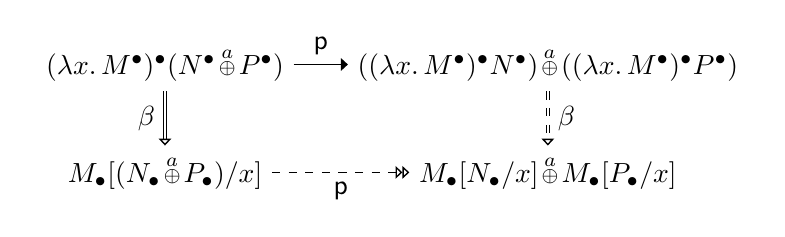
\begin{tikzpicture}
	\matrix[matrix of math nodes] (m) {
	  		\trm{(\x.M*)*(N* +a P*)} &[20pt] \trm{((\x.M*)*N*) +a ((\x. M*)*P*)}
	\\[20pt]\trm{Mo[(No +a Po)/x]} & \trm{Mo[No/x] +a Mo[Po/x]}
	\\ };
	\draw[rwb] (m-1-1) --node[above]{$\perm$} (m-1-2);
	\draw[rwp] (m-1-1) --node[left] {$\beta$} (m-2-1);
	\draw[rwp,implied] (m-1-2) --node[right]{$\beta$} (m-2-2);
	\draw[rws,implied] (m-2-1) --node[below]{$\perm$} (m-2-2);
\end{tikzpicture}}}
&	(x\in\fv M)
\\ \\
\vcenter{\hbox{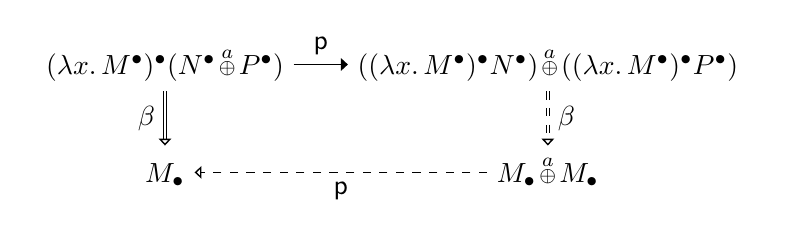
\begin{tikzpicture}
	\matrix[matrix of math nodes] (m) {
	  		\trm{(\x.M*)*(N* +a P*)} &[20pt] \trm{((\x.M*)*N*) +a ((\x. M*)*P*)}
	\\[20pt]\trm{Mo}\vphantom{\trm{+a}} & \trm{Mo +a Mo}
	\\ };
	\draw[rwb] (m-1-1) --node[above]{$\perm$} (m-1-2);
	\draw[rwp] (m-1-1) --node[left] {$\beta$} (m-2-1);
	\draw[rwp,implied] (m-1-2) --node[right]{$\beta$} (m-2-2);
	\draw[rw, implied] (m-2-2) --node[below]{$\perm$} (m-2-1);
\end{tikzpicture}}}
&	(x\notin\fv M)
\end{array}
\]
\end{proof}

How the critical pairs in the above diagrams are joined shows that we cannot use the Hindley-Rosen Lemma \cite[Prop. 3.3.5]{Barendregt84} to prove confluence of $\rw_\beta \cup \rw_\perm$.


\begin{lem}
\label{lem:exhaustive p - parallel beta}
$\trm{No}=_\perm N_{\perm\1}$.
\end{lem}

\begin{proof}
Using \Cref{lem:parallel p-reduction} we decompose $\trm{N*}\rwn_\perm\trm{N*p}$ as
\[
	\trm{N*}=\trm{N_1*}\rwb_\perm\trm{N_2*}\rwb_\perm \dots \rwb_\perm \trm{N_n*}=\trm{N*p}
\]
where $\trm{(N_i)o}=_\perm\trm{(N_{i+1})o}$ by \Cref{lem:parallel p - parallel beta}.
\end{proof}

\subsection{Complete Reduction}

To obtain a reduction strategy with the diamond property for $\rw$, we combine parallel reduction $\rwp_\beta$ with permutative reduction to normal form $\rwn_\perm$ into a notion of \emph{complete reduction} $\rwp$. We will show that it is diamond (\Cref{lem:complete diamond}), and that any step in $\rw$ maps onto a complete step of $\perm$-normal forms (\Cref{lem:p to complete reduction}). Confluence of $\rw$ (\Cref{thm:confluence}) then follows: any two paths $\rws$ map onto complete paths $\rwps$ on $\perm$-normal forms, which then converge by the diamond property.

\begin{defn}
A \emph{complete} reduction step $N\rwp\trm{Nq}$ is a parallel $\beta$-step followed by $\perm$-reduction to normal form:
\[
	N\rwp \trm{Nq} \quad\coloneq\quad N\rwp_\beta \trm{No} \rwn_\perm \trm{Nq}~.
\]
\end{defn}

\begin{lem}[Complete reduction is diamond]
\label{lem:complete diamond}
	If $P\rwpleft N\rwp M$ then for some $Q$, $P\rwp Q\rwpleft M$.
\end{lem}

\begin{proof}
By the following diagram, where $M=N_{\0\perm}$ and $P=N_{\1\perm}$, and $Q=N_{\0\1\perm}$. The square top left is by \Cref{lem:parallel diamond}, top right and bottom left are by \Cref{lem:exhaustive p - parallel beta}, and bottom right is by confluence and strong normalization of $\perm$-reduction.
\[
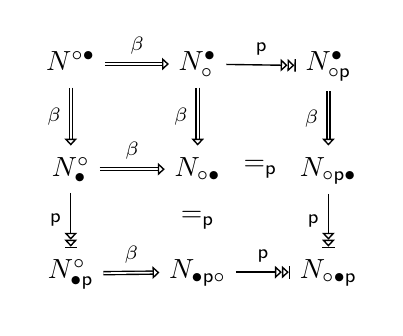
\begin{tikzpicture}
	\matrix (m) [matrix of math nodes] {
	  \trm{N^{\0\1}} &[20pt] & \trm{N_\0^\1} &[20pt] & \trm{N_{\0\perm}^\1} \\[20pt]
	  \\
	  \trm{N_\1^\0}	&& \trm{N_{\0\1}} && \trm{N_{\0\perm\1}} \\[20pt]
		\\
	  \trm{N_{\1\perm}^\0} && \trm{N_{\1\perm\0}} && \trm{N_{\0\1\perm}} \\
	};
	\draw[rwp] (m-1-1) --node[above]{$\scriptstyle\beta$} (m-1-3);
	\draw[rwp] (m-1-1) --node[left] {$\scriptstyle\beta$} (m-3-1);
	\draw[rwp] (m-1-3) --node[left] {$\scriptstyle\beta$} (m-3-3);
	\draw[rwp] (m-3-1) --node[above]{$\scriptstyle\beta$} (m-3-3);
	%
	\draw[rwn] (m-1-3) --node[above]{$\scriptstyle\perm$} (m-1-5);
	\draw[rwn] (m-3-1) --node[left] {$\scriptstyle\perm$} (m-5-1);
	\draw[rwp] (m-5-1) --node[above]{$\scriptstyle\beta$} (m-5-3);
	\draw[rwp] (m-1-5) --node[left] {$\scriptstyle\beta$} (m-3-5);
	%
	\path (m-3-3) --node{$=_\perm$} (m-3-5);
	\path (m-3-3) --node{$=_\perm$} (m-5-3);
	\draw[rwn] (m-5-3) --node[above]{$\scriptstyle\perm$} (m-5-5);
	\draw[rwn] (m-3-5) --node[left] {$\scriptstyle\perm$} (m-5-5);
\end{tikzpicture}
\]
\end{proof}

\begin{lem}
[$\perm$-Normalization maps reduction to complete reduction]%
\label{lem:p to complete reduction}%
If $N\rw M$ then $N_\perm\rwp M_\perm$.
\end{lem}

\begin{proof}
For a $\perm$-step $N\rw_\perm M$ we have $N_\perm=M_\perm$ while $\rwp_\beta$ is reflexive.
For a $\beta$-step $N\rw_\beta M$ we label the reduced redex in $N$ to get $\trm{N*}\rwp_\beta\trm{No}=M$. Then \Cref{lem:exhaustive p - parallel beta} gives $N_{\perm\1}=_\perm M$, and hence $\trm{Np}\rwp_\beta N_{\perm\1}\rwn_\perm M_\perm$.
\end{proof}


\begin{figure}[!t]
  \fbox{
      \begin{minipage}{.97\textwidth}
      \vspace{-4pt}
        \[
        \begin{array}{c@{\qquad}c@{\qquad}c@{\qquad}c}
          \vcenter{\hbox{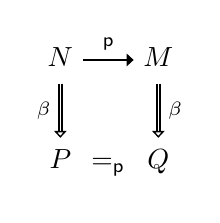
\begin{tikzpicture}
	        \matrix (m) [matrix of math nodes,ampersand replacement=\&] {
	          \trm{N} \&\& \trm{M} \\[20pt] \\ \trm{P} \& =_\perm \& \trm{Q} \\
	        };
	        \draw[rwb] (m-1-1) --node[above]{$\scriptstyle\perm$} (m-1-3);
	        \draw[rwp] (m-1-1) --node[left] {$\scriptstyle\beta$} (m-3-1);
	        \draw[rwp] (m-1-3) --node[right]{$\scriptstyle\beta$} (m-3-3);
          \end{tikzpicture}}}
          &
          \vcenter{\hbox{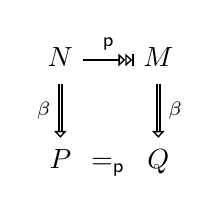
\begin{tikzpicture}
	        \matrix (m) [matrix of math nodes,ampersand replacement=\&] {
	          \trm{N} \&\& \trm{M} \\[20pt] \\ \trm{P} \& =_\perm \& \trm{Q} \\
	        };
	        \draw[rwn] (m-1-1) --node[above]{$\scriptstyle\perm$} (m-1-3);
	        \draw[rwp] (m-1-1) --node[left] {$\scriptstyle\beta$} (m-3-1);
	        \draw[rwp] (m-1-3) --node[right]{$\scriptstyle\beta$} (m-3-3);
          \end{tikzpicture}}}
          &
          \vcenter{\hbox{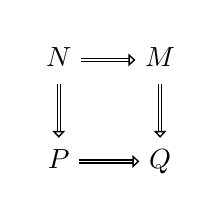
\begin{tikzpicture}
	        \matrix (m) [matrix of math nodes,ampersand replacement=\&] {
	          \trm{N} \&[20pt] \& \trm{M} \\[20pt] \\ \trm{P} \&\& \trm{Q} \\
	        };
	        \draw[rwp] (m-1-1) -- (m-1-3);
	        \draw[rwp] (m-1-1) -- (m-3-1);
	        \draw[rwp] (m-1-3) -- (m-3-3);
	        \draw[rwp] (m-3-1) -- (m-3-3);
          \end{tikzpicture}}}
          &
          \vcenter{\hbox{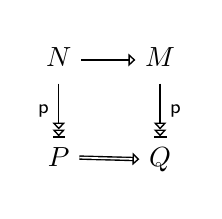
\begin{tikzpicture}
	        \matrix (m) [matrix of math nodes,ampersand replacement=\&] {
	          \trm{N} \&[20pt] \& \trm{M} \\[20pt] \\ P \&\& Q \\
	        };
	        \draw[rw]  (m-1-1) -- (m-1-3);
	        \draw[rwn] (m-1-1) --node[left] {$\scriptstyle\perm$} (m-3-1);
	        \draw[rwn] (m-1-3) --node[right]{$\scriptstyle\perm$} (m-3-3);
	        \draw[rwp] (m-3-1) -- (m-3-3);
          \end{tikzpicture}}}
          \\ \\
          \text{\Cref{lem:parallel p - parallel beta}}
          & \text{\Cref{lem:exhaustive p - parallel beta}}
          & \text{\Cref{lem:complete diamond}}
          & \text{\Cref{lem:p to complete reduction}}
          \\[4pt]
        \end{array}
        \]
    \end{minipage}}
  \caption{Diagrams for the Lemmata Leading up to Confluence}
  \label{fig:confluence diagrams}
\end{figure}

\begin{thm}
\label{thm:confluence}
Reduction $\rw$ is confluent.
\end{thm}

\begin{proof}
By the following diagram. For the top and left areas, by Lemma~\ref{lem:p to complete reduction} any reduction path $N\rws M$ maps onto one $N_\perm \rwx M_\perm$. The main square follows by the diamond property of complete reduction, \Cref{lem:complete diamond}.

\[
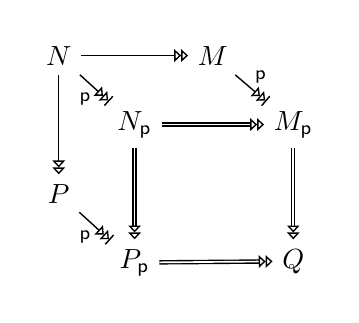
\begin{tikzpicture}
	\matrix (m) [matrix of math nodes] {
	  N &[10pt] &[10pt] M &[10pt] \\[10pt] & N_\perm && M_\perm \\[10pt] P \\[10pt] & P_\perm && Q \\
	};
	\draw[rws] (m-1-1) -- (m-1-3);
	\draw[rws] (m-1-1) -- (m-3-1);
	\draw[rwn] (m-1-1) --node[below left =-2pt] {$\scriptstyle\perm$} (m-2-2);
	\draw[rwn] (m-1-3) --node[above right=-2pt]{$\scriptstyle\perm$} (m-2-4);
	\draw[rwn] (m-3-1) --node[below left =-2pt] {$\scriptstyle\perm$} (m-4-2);
	\draw[rwx] (m-2-2) -- (m-2-4);
	\draw[rwx] (m-2-2) -- (m-4-2);
	\draw[rwx] (m-2-4) -- (m-4-4);
	\draw[rwx] (m-4-2) -- (m-4-4);
\end{tikzpicture}
\]
\end{proof}


%=====================================================================================

\section{Strong Normalization for Simply-Typed Terms}
\label{sec:SN}

In this section, we prove that the relation $\rw$ enjoys strong
normalization in \emph{simply typed} terms. Our proof of strong
normalization is based on the classic reducibility technique,
and inherently has to deal with label-open terms. It thus make great
sense to turn the order $<_{{\trm{M}}}$ from
Definition~\ref{def:orderlabels} into something more formal, at the same time
allowing terms to be label-\emph{open}. 
This is in Figure~\ref{fig:order}.
%
\begin{figure}[!t]
  \fbox{
    \begin{minipage}{.97\textwidth}
    \vspace{4pt}
      \begin{tabular}{ll}
        \textsf{Label Sequences}: & $\theta\quad\coloneqq\quad \varepsilon ~\mid~ a\cdot\theta$\\[5pt]
        \textsf{Label Judgments}: & $\xi\quad\coloneqq\quad \labjudg{\theta}{M}$\\
        \begin{minipage}{.25\textwidth}\textsf{Label Rules}:\end{minipage} &
        \begin{minipage}{.70\textwidth}
        \[
        \begin{array}{c}
        \infer{\labjudg{\theta}{x}}{}\qquad\quad
        \infer{\labjudg{\theta}{\x.M}}{\labjudg{\theta}{M}}\qquad\quad
        \infer{\labjudg{\theta}{\ttrm{!a.M}}}{\labjudg{a\cdot\theta}{M}}
        \\\\
        \infer{\labjudg{\theta}{MN}}{\labjudg{\theta}{M} & \labjudg{\theta}{N}}\qquad\quad
        \infer{\labjudg{\theta}{\ttrm{M +a N}}}{\labjudg{\theta}{M} & \labjudg{\theta}{N} & a\in\theta}
        \end{array}
        \]
        \end{minipage}
        \\
      \end{tabular}
      \vspace{4pt}
    \end{minipage}}
  \caption{Labeling Terms}
    \label{fig:order}
\end{figure}
%
It is easy to realize that, of course modulo label $\alpha$-equivalence, for
every term $M$ there is at least one $\theta$ such that $\labjudg{\theta}{M}$.
An easy fact to check is that if $\labjudg{\theta}{M}$ and $M\rw N$, then $\labjudg{\theta}{N}$.
It thus makes sense to parametrize $\rw$ on a sequence
of labels $\theta$, \ie, one can define a family of reduction
relations $\rw^\theta$ on pairs in the form $(M,\theta)$.
The set of strongly normalizable terms, and the number of steps
to normal forms become themselves parametric:
\begin{varitemize}
\item
  The set $\mathit{SN}^\theta$ of those terms $M$ such
  that $\labjudg{\theta}{M}$ and $(M,\theta)$ is strongly
  normalizing modulo $\rw^\theta$;
\item
  The function $\mathit{sn}^\theta$ assigning to any
  term in $\mathit{SN}^\theta$ the maximal number of $\rw^\theta$
  steps to normal form.
\end{varitemize}

\noindent
We can now define types, environments, judgments, and typing rules in
Figure~\ref{fig:typing}.

\begin{figure}
  \fbox{
    \begin{minipage}{.97\textwidth}
    \vspace{4pt}
      \begin{tabular}{ll@{}l}
        \textsf{Types}: & $\tau$ & $\quad\coloneqq\quad \alpha ~\mid~ \tau\arrow\rho$\\[5pt]
        \textsf{Environments}: & $\Gamma$ & $\quad\coloneqq\quad x_1:\tau_1,\ldots,x_n:\tau_n$\\[5pt]
        \textsf{Judgments}: & $\pi$ & $\quad\coloneqq\quad \judg{\Gamma}{M}{\tau}$\\
        \begin{minipage}{.20\textwidth}\textsf{Typing Rules}:\end{minipage} &
        \multicolumn{2}{@{}c@{}}{
        \begin{minipage}{.75\textwidth}
        \[
        \begin{array}{@{}c@{}}
        \infer{\judg{\Gamma,x:\tau}{x}{\tau}}{}\qquad\quad
        \infer{\judg{\Gamma}{\x.M}{\tau\arrow\rho}}{\judg{\Gamma,x:\tau}M\rho}\qquad\quad
        \infer{\judg{\Gamma}{\ttrm{!a.M}}{\tau}}{\judg{\Gamma}{M}{\tau}}
        \\\\
        \infer{\judg{\Gamma}{MN}{\rho}}{\judg{\Gamma}{M}{\tau\arrow\rho} & \judg{\Gamma}{N}{\tau}}\qquad\quad
        \infer{\judg{\Gamma}{\ttrm{M +a N}}{\tau}}{\judg{\Gamma}{M}{\tau} & \judg{\Gamma}{N}{\tau}}
        \end{array}
        \]
        \end{minipage}}
        \\
      \end{tabular}
      \vspace{4pt}
    \end{minipage}%
  }
  \caption{Types, Environments, Judgments, and Rules}
  \label{fig:typing}
\end{figure}
Please notice that the type structure is precisely the one of the
usual, vanilla, simply-typed $\lambda$-calculus (although terms are of
course different), and we can thus reuse most of the usual proof of
strong normalization, for example in the version given by Ralph
Loader's notes~\cite{Loader98}, page 17.

\begin{lem}\label{lemma:closure}
The closure rules in Figure~\ref{fig:rules} are all sound.
\end{lem}

\begin{figure}[!t]
    \fbox{
      \begin{minipage}{.97\textwidth}
      \vspace{10pt}
        $\quad
        \infer{xL_1\ldots L_m\in\mathit{SN}^\theta}{L_1\in\mathit{SN}^\theta &\cdots & L_m\in\mathit{SN}^\theta}
        \hfill
        \infer{\trm{M +a N}L_1 \ldots L_m\in\mathit{SN}^\theta}{ML_1\ldots L_m\in\mathit{SN}^\theta & NL_1\ldots L_m\in\mathit{SN}^\theta & a\in\theta}
        \quad$
        \\[15pt]
        ${}\quad
    	\infer{\trm{(\x.M)}L_0\ldots L_m\in\mathit{SN}^\theta}{\trm{M[L_0/x]}L_1\ldots L_m\in\mathit{SN}^\theta & L_0\in\mathit{SN}^\theta}
        \hfill
        \infer{\trm{(!a.M)}L_1\ldots L_m\in\mathit{SN}^\theta}{\trm{M}L_1\ldots L_m\in\mathit{SN}^{a\cdot\theta} & \forall i.a\not\in L_i}    
        \quad$
      \vspace{10pt}
      \end{minipage}%
    }
    \caption{Closure Rules for Sets $\mathit{SN}^\theta$}
    \label{fig:rules}
  \end{figure}


Since the structure of the type system is the one of plain, simple
types, the definition of reducibility sets is the classic one:
\begin{align*}
  \RedSet{\alpha}&=\{(\Gamma,\theta,M)\mid M\in\mathit{SN}^\theta\wedge\judg{\Gamma}{M}{\alpha}\};\\
  \RedSet{\tau\arrow\rho}&=\{(\Gamma,\theta,M)\mid(\judg{\Gamma}{M}{\tau\arrow\rho})\wedge(\labjudg{\theta}{M}) \ \wedge\\
    &\qquad\forall(\Gamma\Delta,\theta,N)\in\RedSet{\tau}.(\Gamma\Delta,\theta,MN)\in\RedSet{\rho}\}.
\end{align*}
Before proving that all terms are reducible, we need some
auxiliary results.
\begin{lem}\label{lemma:redprop}
  \begin{enumerate}
  \item\label{point:impl}
    If $(\Gamma,\theta,M)\in\RedSet{\tau}$, then $M\in\mathit{SN}^\theta$.
  \item\label{point:headvar}
    If $\judg{\Gamma}{x L_1\ldots L_m}{\tau}$ and $L_1,\ldots,L_m\in\mathit{SN}^\theta$,
    then $(\Gamma,\theta,x L_1\ldots L_m)\in\RedSet{\tau}$.
  \item\label{point:beta}
    If $(\Gamma,\theta,\trm{M[L_0/x]}L_1\ldots L_m)\in\RedSet{\tau}$
    with $\judg{\Gamma}{L_0}{\rho}$ and $L_0\in\mathit{SN}^\theta$,
    then $(\Gamma,\theta,\trm{(\x.M)}L_0\ldots L_m)\in\RedSet{\tau}$.
  \item\label{point:sum}
    If $(\Gamma,\theta,ML_1\ldots L_m)\in\RedSet{\tau}$ with
    $(\Gamma,\theta,NL_1\ldots L_m)\in\RedSet{\tau}$ and $a\in\theta$,
    then $(\Gamma,\theta,\trm{(M +a N)}L_1\ldots L_m)\in\RedSet{\tau}$.
  \item\label{point:box}
    \begin{sloppypar}
    If $(\Gamma,a\cdot\theta,ML_1\ldots L_m)\in\RedSet{\tau}$
    and $a\not\in L_i$ for all $i$,\\
    then $(\Gamma,\theta,\trm{(!a.M)}L_1\ldots L_m)\in\RedSet{\tau}$.
    \end{sloppypar}
  \end{enumerate}
\end{lem}
\begin{proof}
  The proof is an induction on $\tau$:
  If $\tau$ is an atom $\alpha$, then Point \ref{point:impl} follows
  by definition, while points \ref{point:headvar} to \ref{point:box}
  come from Lemma~\ref{lemma:closure}.
  If $\tau$ is $\rho\arrow\mu$, Points \ref{point:headvar} to \ref{point:box}
  come directly from the induction hypothesis, while Point \ref{point:impl}
  can be proved by observing that $M$ is in $\mathit{SN}^\theta$
  if $Mx$ is itself $\mathit{SN}^\theta$, where $x$ is a fresh variable.
  By induction hypothesis (on Point~\ref{point:headvar}), we can
  say that $(\Gamma(x:\rho),\theta,x)\in\RedSet{\rho}$, and
  conclude that $(\Gamma(x:\rho),\theta,Mx)\in\RedSet{\mu}$.
\end{proof}

The following is the so-called Main Lemma:
\begin{prop}\label{lemma:mainlemma}
  Suppose $\judg{y_1:\tau_1,\ldots,y_n:\tau_n}{M}{\rho}$ and
  $\labjudg{\theta}{M}$, with
  $(\Gamma,\theta,N_j)\in\RedSet{\tau_j}$ for all $1\leq j\leq
  n$. Then
  $(\Gamma,\theta,M[N_1/y_1,\ldots,N_n/y_n])\in\RedSet{\rho}$.
\end{prop}
\begin{proof}
  This is an induction on the structure of the term $M$:
  \begin{varitemize}
  \item
    If $M$ is a variable, necessarily one among $y_1,\ldots,y_n$,
    then the result is trivial.
  \item
    If $M$ is an application $LP$, then there exists
    a type $\xi$ such that
    $\judg{y_1:\tau_1,\ldots,y_n:\tau_n}{L}{\xi\arrow\rho}$
    and $\judg{y_1:\tau_1,\ldots,y_n:\tau_n}{P}{\xi}$. Moreover,
    $\labjudg{\theta}{L}$ and $\labjudg{\theta}{P}$ we can
    then safely apply the induction hypothesis and conclude
    that
    $$
    (\Gamma,\theta,L[\overline{N}/\overline{y}])\in\RedSet{\xi\arrow\rho}
    \qquad
    (\Gamma,\theta,P[\overline{N}/\overline{y}])\in\RedSet{\xi}~.
    $$
    By definition, we get
    $$
    (\Gamma,\theta,(LP)[\overline{N}/\overline{y}])\in\RedSet{\rho}~.
    $$
  \item
    \begin{sloppypar}
    If $M$ is an abstraction $\trm{\x.L}$, then $\rho$
    is an arrow type $\xi\arrow\mu$ and
    $\judg{y_1:\tau_1,\ldots,y_n:\tau_n,x:\xi}{L}{\mu}$.
    Now, consider any $(\Gamma\Delta,\theta,P)\in\RedSet{\xi}$.
    Our objective is to prove with this hypothesis
    that $(\Gamma\Delta,\theta,(\x.L[\overline{N}/\overline{y}])P)\in\RedSet{\mu}$.
    By induction hypothesis, since $(\Gamma\Delta,N_i)\in\RedSet{\tau_i}$,
    we get that $(\Gamma\Delta,\theta,L[\overline{N}/\overline{y},P/x])\in\RedSet{\mu}$.
    The thesis follows from Lemma~\ref{lemma:redprop}.
    \end{sloppypar}
  \item
    If $M$ is a sum $\trm{L+a P}$, we can make use of Lemma~\ref{lemma:redprop}
    and the induction hypothesis, and conclude.
  \item
    If $M$ is a generator $\trm{!a.P}$, we can make use of Lemma~\ref{lemma:redprop}
    and the induction hypothesis. We should however observe that $\labjudg{a\cdot\theta}{P}$,
    since $\labjudg{\theta}{M}$.
  \end{varitemize}
\end{proof}

We now have all the ingredients for our proof of strong normalization:
\begin{thm}
  If $\judg{\Gamma}{M}{\tau}$ and $\labjudg{\theta}{M}$, then $M\in\mathit{SN}^\theta$.
\end{thm}
\begin{proof}
  Suppose that $\judg{x_1:\rho_1,\ldots,x_n:\rho_n}{M}{\tau}$.
  Since $\judg{x_1:\rho_1,\ldots,x_n:\rho_n}{x_i}{\rho_i}$ for all
  $i$, and clearly $\labjudg{\theta}{x_i}$ for every $i$, we
  can apply Lemma \ref{lemma:mainlemma} and
  obtain that $(\Gamma,\theta,M[\overline{x}/\overline{x}])\in\RedSet{\tau}$
  from which, via Lemma~\ref{lemma:redprop}, one gets the thesis.
\end{proof}

%============================================================ PROJECTIVE


\section{Projective Reduction}
\label{sec:projective-reduction}

Permutative reduction $\rw_\perm$ evaluates probabilistic sums purely by rewriting. Here we look at a more standard \emph{projective} notion of reduction, which conforms more closely to the intuition that $\ttrm{!a}$ generates a probabilistic event to determine the choice $\ttrm{+a}$. Using $+$ for an external probabilistic sum, we expect to reduce $\ttrm{!a.N}$ to $N_0+N_1$ where each $N_i$ is obtained from $N$ by projecting every subterm $\ttrm{M_0+aM_1}$ to $M_i$. The question is, in what context should we admit this reduction? We first limit ourselves to reducing in \emph{head} position.

\begin{defn}
The \emph{$a$-projections} $\proj a0N$ and $\proj a1N$ are defined as follows:
\begin{align*}
	\proj a0{N+aM} &= \proj a0N		&	\proj ai{\x.N} &= \x.\proj aiN
\\	\proj a1{N+aM} &= \proj a1M		&	\proj ai{NM}   &= \proj aiN\,\proj aiM
\\	\proj ai{!a.N} &= \trm{!a.N}	& 	\proj ai{N+bM} &= \proj aiN\,\trm{+b}\,\proj aiM && \text{if } a \neq b
\\	\proj aix      &= x				&	\proj ai{!b.N} &= \trm{!b.}\proj aiN 			 && \text{if } a \neq b.
\end{align*}
\end{defn}

\begin{defn}
A \emph{head context} $H[\,]$ is given by the following grammar.
\[
	H[\,] \coloneqq [\,] ~\mid~ \x.\,H[\,] ~\mid~ H[\,]N
\]
\end{defn}

\begin{defn}
\label{defn:projective head reduction}
\emph{Projective head reduction} $\rw_\ph$ is given by
\[
	\trm{H[\,!a.N]} ~\rw_\ph~ H[\proj a0N] + H[\proj a1N]~.
\]
\end{defn}

We can simulate $\rw_\ph$ by permutative reduction if we interpret the external sum $+$ by an outermost $\+$ (taking special care if the label does not occur).

\begin{prop}
\label{prop:permutative-simulates-projective}
Permutative reduction simulates projective head reduction:
\[
	H[\,\trm{!a.N}] ~\rws_\perm~
	\left\{\begin{array}{l@{\qquad}l}
		H[N]						 & \text{if }a\notin\fl N \\[5pt]
		H[\proj a0N] \+ H[\proj a1N] & \text{otherwise}.
	\end{array}\right.
\]
\end{prop}

\begin{proof}
The case $a\notin\fl N$ is immediate by a $\boxVoid$ step. For the other case, observe that $\trm{H[\,!a.N]}\rws_\perm\trm{!a.H[N]}$ by $\boxAbs$ and $\boxFun$ steps, and since $a$ does not occur in $H[\,]$, that $H[\proj aiN]=\proj ai{H[N]}$. By induction on $N$, if $a$ is minimal in $N$ (\ie\ $a\in\fl N$ and $a\leq b$ for all $b\in\fl N$) then $N\rws_\perm \proj a0N\trm{+a}\proj a1N$. As required,
\[
	H[\,\trm{!a.N}]~\rws_\perm~ \trm{!a.}\,H[\proj a0N]\, \trm{+a}\, H[\proj a1N] \quad\text{if }a\in\fl N~.
\]
\end{proof}

A gap remains between which generators will not be duplicated, which we \emph{should} be able to reduce, and which generators projective head reduction \emph{does} reduce. In particular, to interpret call-by-value probabilistic reduction in Section~\ref{sec:cbv}, we would like to reduce under other generators. However, permutative reduction does not permit exchanging generators, and so only simulates reducing in head position. While (independent) probabilistic events are generally considered interchangeable, it is a question whether the below equivalence is desirable.
%
\begin{align}
\label{eqn:permute-generators}
	\trm{!a.!b.N} \quad\smash{\stackrel?\sim}\quad \trm{!b.!a.N}
\end{align}
%
We elide the issue by externalizing probabilistic events, and reducing with reference to a predetermined binary stream $s\in\{0,1\}^{\mathbb N}$ representing their outcomes. In this way, we will preserve the intuitions of both permutative and projective reduction: we obtain a qualified version of the equivalence~\eqref{eqn:permute-generators} (see \eqref{eqn:permute-generators-streams} below), and will be able to reduce any generator on the \emph{spine} of a term: under (other) generators and choices as well as under abstractions and in function position.

\begin{defn}
The set of \emph{streams} is $\Streams=\{0,1\}^\mathbb{N}$, ranged over by $r,s,t$, and $i\cdot s$ denotes a stream with $i\in\{0,1\}$ as first element and $s$ as the remainder.
\end{defn}

\begin{defn}
The \emph{stream labeling} $N^s$ of a term $N$ with a stream $s\in\Streams$, which annotates generators as $\trm{!ai}$ with $i\in\{0,1\}$ and variables as $x^s$ with a stream $s$, is given inductively below. We lift $\beta$-reduction to stream-labeled terms by introducing a substitution case for stream-labeled variables: $x^s[M/x] = M^s$.
\begin{align*}
	\trm{(\x.N)^s} &= \trm{\x.N^s} & \trm{(!a.N)^{i\cdot s}} &= \trm{!ai.N^s} 
	\\
	\trm{(N\,M)^s} &= \trm{N^s\,M} & \trm{(N+a M)^s}		 &= \trm{N^s +a M^s}
\end{align*}
\end{defn}

\begin{defn}
\emph{Projective reduction} $\rw_\pi$ on stream-labeled terms is the rewrite relation given by
\[
	\trm{!ai.N} ~\rw_\pi~\proj aiN~.
\]
\end{defn}

Observe that in $N^s$ a generator that occurs under $n$ other generators on the spine of $N$, is labeled with the element of $s$ at position $n+1$. Generators in argument position remain unlabeled, until a $\beta$-step places them on the spine, in which case they become labeled by the new substitution case. We allow to annotate a term with a finite prefix of a stream, \eg\ $N^i$ with a singleton $i$, so that only part of the spine is labeled. Subsequent labeling of a partly labeled term is then by $(N^r)^s=N^{r\cdot s}$ (abusing notation). To introduce streams via the external probabilistic sum, and to ignore an unused remaining stream after completing a probabilistic computation, we adopt the following equation.
\[
 	N = N^0 + N^1
\]

\begin{prop}
Projective reduction generalizes projective head reduction:
\[
	\trm{H[\,!a.N]} ~=~ \trm{H[\,!a{}^0.N]} + \trm{H[\,!a{}^1.N]} ~\rw_\pi~ H[\proj a0N]+H[\proj a1N]~.
\]
\end{prop}

Returning to the interchangeability of probabilistic events, we refine~\eqref{eqn:permute-generators} by exchanging the corresponding elements of the annotating streams:
\begin{align}
\label{eqn:permute-generators-streams}
\vcenter{\hbox{
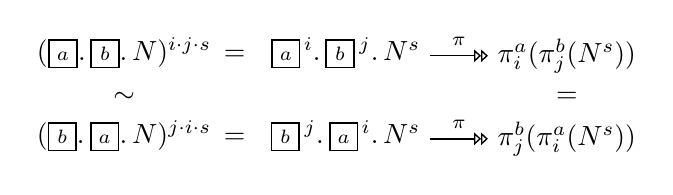
\begin{tikzpicture}[x=80pt,y=-15pt]
	\node     at (0,0) {$\trm{(!a.!b.N)}^{i\cdot j\cdot s}$};
	\node     at (0,2) {$\trm{(!b.!a.N)}^{j\cdot i\cdot s}$};
	\node (A) at (1,0) {$\trm{!ai.!b{}^j.N^s}$};
	\node (B) at (1,2) {$\trm{!b{}^j.!ai.N^s}$};
	\node (C) at (2,0) {$\pi^a_i(\proj bj{N^s})$};
	\node (D) at (2,2) {$\pi^b_j(\proj ai{N^s})$};
	\draw[rws] (A) --node[above] {$\scriptstyle\pi$}   (C);
	\draw[rws] (B) --node[above]{$\scriptstyle\pi$}   (D);
	\node at (0,1) {$\sim$};
	\node at (0.5,0) {$=$};
	\node at (0.5,2) {$=$};
	\node at (2,1) {$=$};
\end{tikzpicture}}}
\end{align}

Stream-labeling externalizes all probabilities, making reduction deterministic. This is expressed by the following proposition, that stream-labeling commutes with reduction: if a generator remains unlabeled in $M$ and becomes labeled after a reduction step $M\rw N$, what label it receives is predetermined. The deep reason is that stream labeling assigns an outcome to each generator in a way that corresponds to a call-by-name strategy for probabilistic reduction.


\begin{prop}
\label{prop:labeling-commutes}
If $M \rw N$ by a step other than $\boxVoid$ then $M^s \rw N^s$.
\end{prop}

\begin{rmrk}
The statement is false for the $\boxVoid$ rule $\trm{!a.N}\rw_\perm N~(a\notin\fl N)$, as it removes a generator but not an element from the stream. Arguably, for this reason the rule should be excluded from the calculus. On the other hand, the rule is necessary to implement idempotence of $\+$, rather than just $\ttrm{+a}$, as follows.
\[
	N\+N ~=~ \trm{!a.N+aN} ~\rw_\perm~ \trm{!a.N} ~\rw_\perm~ N \qquad \text{where } a\notin\fl N
\]
\end{rmrk}

The below proposition then expresses that projective reduction is an \emph{invariant} for permutative reduction. If $N\rw_\perm M$ by a step (that is not $\boxVoid$) on a labeled generator $\ttrm{!ai}$ or a corresponding choice $\ttrm{+a}$, then $N$ and $M$ reduce to a common term, $N\rw_\pi P\,{}_\pi\lw\,M$, by the projective steps evaluating $\ttrm{!ai}$.

\begin{prop}
Projective reduction is an invariant for permutative reduction, as follows (with a case for $\cancelR$ symmetric to $\cancelL$, and where $D[\,]$ is a context).
\[
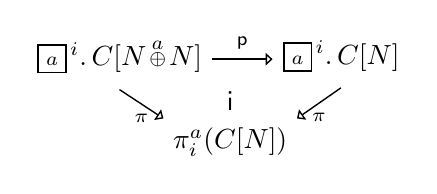
\begin{tikzpicture}[x=40pt,y=30pt]
	\node (A) at (0,1) {$\trm{!ai.C[N+aN]}$};
	\node (B) at (2,1) {$\trm{!ai.C[N]}$};
	\node (C) at (1,0) {$\proj ai{C[N]}$};
	\draw[rw] (A) --node[above]{$\scriptstyle\perm$} (B);
	\draw[rw] (A.south) --node[below] {$\scriptstyle\pi$}  (C.north west);
	\draw[rw] (B.south) --node[below]{$\scriptstyle\pi$}   (C.north east);
	\node at (1,.5) {$\idem$};
\end{tikzpicture}
\qquad
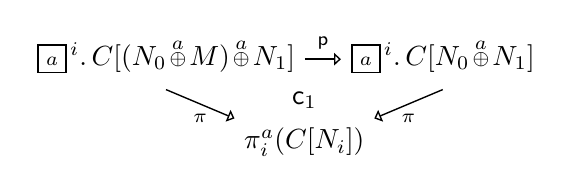
\begin{tikzpicture}[x=50pt,y=30pt]
	\node (A) at (0,1) {$\trm{!ai.C[(N_0 +a M) +a N_1]}$};
	\node (B) at (2,1) {$\trm{!ai.C[N_0 +a N_1]}$};
	\node (C) at (1,0) {$\proj ai{C[N_i]}$};
	\draw[rw] (A) --node[above]{$\scriptstyle\perm$} (B);
	\draw[rw] (A.south) --node[below] {$\scriptstyle\pi$}  (C.north west);
	\draw[rw] (B.south) --node[below]{$\scriptstyle\pi$}   (C.north east);
	\node at (1,.5) {$\cancelL$};
\end{tikzpicture}
\]
\[
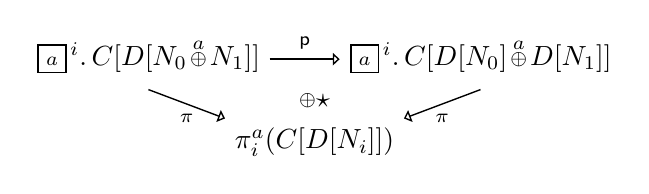
\begin{tikzpicture}[x=60pt,y=30pt]
	\node (A) at (0,1) {$\trm{!ai.C[D[N_0+aN_1]]}$};
	\node (B) at (2,1) {$\trm{!ai.C[D[N_0]+aD[N_1]]}$};
	\node (C) at (1,0) {$\proj ai{C[D[N_i]]}$};
	\draw[rw] (A) --node[above]{$\scriptstyle\perm$} (B);
	\draw[rw] (A.south) --node[below] {$\scriptstyle\pi$}  (C.north west);
	\draw[rw] (B.south) --node[below]{$\scriptstyle\pi$}   (C.north east);
	\node at (1,.5) {$\plusX$};
\end{tikzpicture}
\]
\[
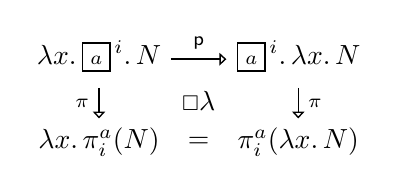
\begin{tikzpicture}[x=36pt,y=30pt]
	\node (A) at (0,1) {$\trm{\x.!ai.N}$};
	\node (B) at (2,1) {$\trm{!ai.\x.N}$};
	\node (C) at (0,0) {$\x.\,\proj aiN$};
	\node (D) at (2,0) {$\proj ai{\x.N}$};
	\draw[rw] (A) --node[above]{$\scriptstyle\perm$} (B);
	\draw[rw] (A) --node[left] {$\scriptstyle\pi$}   (C);
	\draw[rw] (B) --node[right]{$\scriptstyle\pi$}   (D);
	\node at (1,0) {$=$};
	\node at (1,.5) {$\boxAbs$};
\end{tikzpicture}
\qquad\qquad
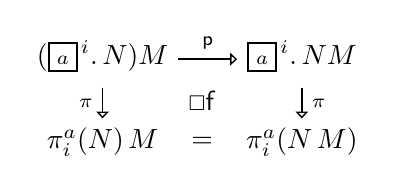
\begin{tikzpicture}[x=36pt,y=30pt]
	\node (A) at (0,1) {$\trm{(!ai.N)M}$};
	\node (B) at (2,1) {$\trm{!ai.NM}$};
	\node (C) at (0,0) {$\proj aiN\,M$};
	\node (D) at (2,0) {$\proj ai{N\,M}$};
	\draw[rw] (A) --node[above]{$\scriptstyle\perm$} (B);
	\draw[rw] (A) --node[left] {$\scriptstyle\pi$}   (C);
	\draw[rw] (B) --node[right]{$\scriptstyle\pi$}   (D);
	\node at (1,0) {$=$};
	\node at (1,.5) {$\boxFun$};
\end{tikzpicture}
\]
\end{prop}


%============================================================ CALL-BY-VALUE

\section{Call-by-value Interpretation}
\label{sec:cbv}

We consider the interpretation of a call-by-value probabilistic $\lambda$-calculus. For simplicity we will allow duplicating (or deleting) $\beta$-redexes, and only restrict duplicating probabilities; our \emph{values} $V$ are then just deterministic---\ie~without choices---terms, possibly applications and not necessarily $\beta$-normal (so that our $\rw_{\beta\val}$ is actually $\beta$-reduction on deterministic terms, unlike \cite{DalLagoZorzi12}). We evaluate the internal probabilistic choice $\ttrm{v{}}$ to an external probabilistic choice $+$.

\begin{align*}
N &\coloneqq x \mid \x.N \mid MN \mid \trm{M v N}  & (\x.N)V 		\rw_{\beta\val} \ & N[V/x]
\\[5pt]
V, W &\coloneqq x \mid \x.V \mid VW  					& \trm{M v N} \, \rw_\val \, \ & M + N
\end{align*}

The interpretation $\uncbv{N}$ of a call-by-value term $N$ into $\PEL$ is given as follows. First, we translate $N$ to a label-open term $\unopen N=\labjudg\theta P$ by replacing each choice $\ttrm{v}$ with one $\ttrm{+a}$ with a unique label, where the label-context $\theta$ collects the labels used. Then $\uncbv{N}$ is the \emph{label closure} $\uncbv{N}=\labclose\theta P$, which prefixes $P$ with a generator $\ttrm{!a}$ for every $a$ in $\theta$.

\begin{defn}(Call-by-value interpretation)
The \emph{open interpretation} $\unopen N$ of a call-by-value term $N$ is as follows, where all labels are fresh, and inductively $\unopen{N_i}=\labjudg{\theta_i}{P_i}$ for $i\in\{1,2\}$.
\[
\begin{array}{r@{\quad}c@{\quad}l@{\qquad}r@{\quad}c@{\quad}l}
		\unopen x 		 &=& \labjudg{}x				& \unopen {N_1N_2}   &=& \labjudg{\theta_2\cdot\theta_1}{P_1P_2}
\\[5pt]	\unopen {\x.N_1} &=& \labjudg{\theta_1}{\x.P_1} & \unopen {N_1\plusval N_2} &=& \labjudg{\theta_2\cdot\theta_1\cdot a}{\trm{P_1 +a P_2}}
\end{array}
\]
The \emph{label closure} $\labclose\theta P$ is given inductively as follows.
\[
	\labclose{}P = P \qquad \labclose{a\cdot\theta}P = \labclose\theta{\trm{!a.P}}
\]
The \emph{call-by-value interpretation} of $N$ is $\uncbv N=\lfloor\unopen N\rfloor$.
\end{defn}

Our call-by-value reduction may choose an arbitrary order in which to evaluate the choices $\ttrm{v{}}$ in a term $N$, but the order of generators in the interpretation $\uncbv N$ is necessarily fixed. Then to simulate a call-by-value reduction, we cannot choose a fixed context stream a priori; all we can say is that for every reduction, there is some stream that allows us to simulate it. Specifically, a reduction step $\trm{C[N_0vN_1]}\rw_\val\trm{C[N_j]}$ where $C[\,]$ is a call-by-value term context is simulated by the following projective step.
\[
	\trm{\dots!ai.!b{}^j.!c{}^k\dots D[P_0+bP_1]}
	\rw_\pi
	\trm{\dots!ai.!c{}^k\dots D[P_j]}
\]
Here, $\unopen{\trm{C[N_0vN_1]}}=\labjudg{\theta}{\trm{D[P_0+bP_1]}}$ with $D[\,]$ a $\PEL$-context, and $\theta$ giving rise to the sequence of generators $\ttrm{\dots!a.!b.!c\dots}$ in the call-by-value translation. To simulate the reduction step, if $b$ occupies the $n$-th position in $\theta$, then the $n$-th position in the context stream $s$ must be the element $j$. Since $\beta$-reduction survives the translation and labeling process intact, we may simulate call-by-value probabilistic reduction by projective and $\beta$-reduction.

\begin{thm}
If $N\rws_{\val,\beta\val}V$ then $\uncbv N^s\rws_{\pi,\beta}\uncbv V$ for some stream $s\in\Streams$.
\end{thm}


\section{Conclusions and Future Work}

We believe our decomposition of probabilistic choice in $\lambda$-calculus to be an elegant and compelling way of restoring confluence, one of the core properties of the $\lambda$-calculus. Our probabilistic event $\lambda$-calculus captures traditional call-by-name and call-by-value probabilistic reduction, and offers finer control beyond those strategies. Permutative reduction implements a natural and fine-grained equivalence on probabilistic terms as internal rewriting, while projective reduction provides a complementary and more traditional external perspective.

There are a few immediate areas for future work. Firstly, within probabilistic $\lambda$-calculus, it is worth exploring if our decomposition opens up new avenues in semantics. Secondly, our approach might apply to probabilistic reasoning more widely, outside the $\lambda$-calculus. Most importantly, we will explore if our approach can be extended to other computational effects. Our use of streams interprets probabilistic choice as a \emph{read} operation from an external source, which means other read operations can be treated similarly. A complementary treatment of \emph{write} operations would allow us to express a considerable range of effects, including input/output and state.

\subsection*{Acknowledgments}

This work was supported by EPSRC Project EP/R029121/1 \emph{Typed Lambda-Calculi with Sharing and Unsharing}.
The first author is partially supported by the ANR project 19CE480014 PPS, the ERC Consolidator Grant 
818616 DIAPASoN, and the MIUR PRIN 201784YSZ5 ASPRA.
We thank the referees for their diligence and helpful comments. 
We are grateful to Chris Barrett and---indirectly---Anupam Das for pointing us to Zantema and Van de Pol's work~\cite{Zantema-Pol-2001}.


\bibliographystyle{splncs04}
\bibliography{biblio}
\addcontentsline{toc}{section}{References}

%%%%% To display Open Access text and logo, Please add below text and copy the cc_by_4-0.eps in the manuscript package %%%

\newpage

\vspace*{\fill}

{\small\medskip\noindent{\bf Open Access} This chapter is licensed under the terms of the Creative Commons\break Attribution 4.0 International License (\url{http://creativecommons.org/licenses/by/4.0/}), which permits use, sharing, adaptation, distribution and reproduction in any medium or format, as long as you give appropriate credit to the original author(s) and the source, provide a link to the Creative Commons license and indicate if changes were made.}

{\small \spaceskip .28em plus .1em minus .1em The images or other third party material in this chapter are included in the chapter's Creative Commons license, unless indicated otherwise in a credit line to the material.~If material is not included in the chapter's Creative Commons license and your intended\break use is not permitted by statutory regulation or exceeds the permitted use, you will need to obtain permission directly from the copyright holder.}

\medskip\noindent
\includegraphics{cc_by_4-0.eps}

\end{document}

